\documentclass[11pt]{article}

\usepackage[margin=1in]{geometry}
\usepackage{booktabs}
\usepackage{longtable}
\usepackage{array}
\usepackage{enumitem}
\usepackage{graphicx}
\usepackage{tikz}
\usepackage[table]{xcolor}
\usepackage{listings}
\usepackage{needspace}
\usepackage{float}
\usepackage[hidelinks]{hyperref}
\usetikzlibrary{arrows.meta,positioning}
\newcommand{\reprofile}{\texttt{train\_}\allowbreak\texttt{ultrawidescaledtail10\_}\allowbreak\texttt{repro.py}}
\lstset{
    basicstyle=\ttfamily\footnotesize,
    breaklines=true,
    columns=fullflexible,
    frame=single,
    backgroundcolor=\color{gray!6},
    showstringspaces=false,
    tabsize=4,
    keepspaces=true
}

\title{CSE 433 Final Project}
\author{Jack Hunter}
\date{\today}

\begin{document}

\maketitle

\section{Model and Performance Analysis}

My final single-model submission is \texttt{UltraWideScaledTail10}, implemented in
\reprofile. I designed the model for the project
constraint of at most 10 weighted layers, where weighted layers are convolutional or
linear modules on the forward path. Batch normalization, activation functions, pooling,
channel gating, residual additions, stochastic depth, and scalar residual parameters are
not counted as weighted layers.

\subsection{Architecture}

The model uses a wide convolutional trunk followed by a low-resolution scaled residual
tail. The central idea is to spend the limited layer budget on high-capacity feature
maps, while placing the extra residual refinement after the spatial resolution has been
reduced. This gives the model high channel capacity without violating the 10-layer
depth limit.

\begin{center}
\begin{tabular}{rlll}
\toprule
\textbf{Count} & \textbf{Module} & \textbf{Type} & \textbf{Purpose} \\
\midrule
1 & \texttt{stem} & Conv2d & Initial RGB projection \\
2 & \texttt{block1.conv1} & Conv2d & Wide feature extraction \\
3 & \texttt{block1.conv2} & Conv2d & Wide feature extraction \\
4 & \texttt{block2.conv1} & Conv2d & 768-channel feature block \\
5 & \texttt{block2.conv2} & Conv2d & 768-channel feature block \\
6 & \texttt{block3.conv} & Conv2d & Low-resolution transition \\
7 & \texttt{tail.conv1} & Conv2d & Grouped residual tail \\
8 & \texttt{tail.conv2} & Conv2d & Grouped residual tail \\
9 & \texttt{tail.conv3} & Conv2d & Dense residual tail \\
10 & \texttt{fc} & Linear & CIFAR-10 classifier \\
\bottomrule
\end{tabular}
\end{center}

The audited model has exactly 10 weighted layers and 21,337,656 parameters. A dummy
forward pass returns logits of shape $(2, 10)$, matching the 10 CIFAR-10 classes.

\subsection{Visual model data flow}

Figure~\ref{fig:dataflow} shows the main data flow through the network for one
CIFAR-10 image. The diagram reports the feature-map shape after each major stage, after
the pooling operation inside that stage has been applied. The largest activation tensor
appears early, before the spatial resolution has been reduced. The later tail operates
on a compact $768 \times 3 \times 3$ tensor, which is why it is an efficient place to
spend the remaining layer budget.

\begin{figure}[ht]
\centering
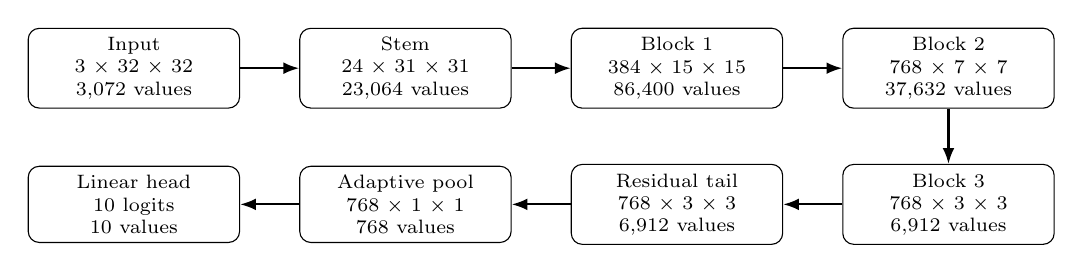
\begin{tikzpicture}[
    node distance=0.7cm and 0.75cm,
    box/.style={draw, rounded corners, align=center, minimum height=0.95cm,
                text width=2.45cm, font=\scriptsize},
    arrow/.style={-{Latex[length=2mm]}, thick}
]
\node[box] (input) {Input\\$3 \times 32 \times 32$\\3,072 values};
\node[box, right=of input] (stem) {Stem\\$24 \times 31 \times 31$\\23,064 values};
\node[box, right=of stem] (b1) {Block 1\\$384 \times 15 \times 15$\\86,400 values};
\node[box, right=of b1] (b2) {Block 2\\$768 \times 7 \times 7$\\37,632 values};

\node[box, below=of b2] (b3) {Block 3\\$768 \times 3 \times 3$\\6,912 values};
\node[box, left=of b3] (tail) {Residual tail\\$768 \times 3 \times 3$\\6,912 values};
\node[box, left=of tail] (pool) {Adaptive pool\\$768 \times 1 \times 1$\\768 values};
\node[box, left=of pool] (fc) {Linear head\\$10$ logits\\10 values};

\draw[arrow] (input) -- (stem);
\draw[arrow] (stem) -- (b1);
\draw[arrow] (b1) -- (b2);
\draw[arrow] (b2) -- (b3);
\draw[arrow] (b3) -- (tail);
\draw[arrow] (tail) -- (pool);
\draw[arrow] (pool) -- (fc);
\end{tikzpicture}
\caption{Visual data flow for \texttt{UltraWideScaledTail10}.}
\label{fig:dataflow}
\end{figure}

\subsection{Layer-by-layer whole-model audit}

Table~\ref{tab:layerdata} gives a forward-pass audit of the whole model, not only the
10 counted weighted layers. The counted project layers are the \texttt{Conv2d} and
\texttt{Linear} rows. The normalization, activation, pooling, channel-gating,
residual-scale, and stochastic-depth rows are included so the table represents the
actual computation path used by the final network. Reused activation modules are
shown at each conceptual use site because this is clearer than hiding repeated GELU
applications behind a single module name.


\begingroup
\scriptsize
\renewcommand{\arraystretch}{1.08}
\setlength{\tabcolsep}{2pt}
\begin{longtable}{@{}r
>{\raggedright\arraybackslash}p{0.16\textwidth}
>{\raggedright\arraybackslash}p{0.10\textwidth}
c
>{\raggedright\arraybackslash}p{0.20\textwidth}
>{\raggedright\arraybackslash}p{0.13\textwidth}
r@{}}
\label{tab:layerdata}\\
\toprule
\rowcolor{gray!18}
\textbf{\#} & \textbf{Layer} & \textbf{Type} & \textbf{Counted?} &
\textbf{Shape / setting} & \textbf{Output} & \textbf{Params} \\
\midrule
\endfirsthead
\caption[]{Whole-model data flow and parameter audit continued.}\\
\toprule
\rowcolor{gray!18}
\textbf{\#} & \textbf{Layer} & \textbf{Type} & \textbf{Counted?} &
\textbf{Shape / setting} & \textbf{Output} & \textbf{Params} \\
\midrule
\endhead
\bottomrule
\endfoot
\bottomrule
\endlastfoot
\rowcolor{gray!5}
1 & \texttt{stem} & Conv2d & Yes & $24{\times}3{\times}2{\times}2$ &
$24{\times}31{\times}31$ & 312 \\
2 & \texttt{stem\_act} & GELU & No & -- &
$24{\times}31{\times}31$ & 0 \\
\rowcolor{gray!5}
3 & \texttt{block1.conv1} & Conv2d & Yes & $384{\times}24{\times}3{\times}3$ &
$384{\times}31{\times}31$ & 82,944 \\
4 & \texttt{block1.pool} & MaxPool2d & No & $k{=}2,\ s{=}2$ &
$384{\times}15{\times}15$ & 0 \\
\rowcolor{gray!5}
5 & \texttt{block1.bn1} & BNBias & No & $C{=}384$ &
$384{\times}15{\times}15$ & 768 \\
6 & \texttt{block1.act1} & GELU & No & -- &
$384{\times}15{\times}15$ & 0 \\
\rowcolor{gray!5}
7 & \texttt{block1.conv2} & Conv2d & Yes & $384{\times}384{\times}3{\times}3$ &
$384{\times}15{\times}15$ & 1,327,104 \\
8 & \texttt{block1.bn2} & BNBias & No & $C{=}384$ &
$384{\times}15{\times}15$ & 768 \\
\rowcolor{gray!5}
9 & \texttt{block1.act2} & GELU & No & -- &
$384{\times}15{\times}15$ & 0 \\
10 & \texttt{block2.conv1} & Conv2d & Yes & $768{\times}384{\times}3{\times}3$ &
$768{\times}15{\times}15$ & 2,654,208 \\
\rowcolor{gray!5}
11 & \texttt{block2.pool} & MaxPool2d & No & $k{=}2,\ s{=}2$ &
$768{\times}7{\times}7$ & 0 \\
12 & \texttt{block2.bn1} & BNBias & No & $C{=}768$ &
$768{\times}7{\times}7$ & 1,536 \\
\rowcolor{gray!5}
13 & \texttt{block2.act1} & GELU & No & -- &
$768{\times}7{\times}7$ & 0 \\
14 & \texttt{block2.conv2} & Conv2d & Yes & $768{\times}768{\times}3{\times}3$ &
$768{\times}7{\times}7$ & 5,308,416 \\
\rowcolor{gray!5}
15 & \texttt{block2.bn2} & BNBias & No & $C{=}768$ &
$768{\times}7{\times}7$ & 1,536 \\
16 & \texttt{block2.act2} & GELU & No & -- &
$768{\times}7{\times}7$ & 0 \\
\rowcolor{gray!5}
17 & \texttt{block3.conv} & Conv2d & Yes & $768{\times}768{\times}3{\times}3$ &
$768{\times}7{\times}7$ & 5,308,416 \\
18 & \texttt{block3.pool} & MaxPool2d & No & $k{=}2,\ s{=}2$ &
$768{\times}3{\times}3$ & 0 \\
\rowcolor{gray!5}
19 & \texttt{block3.bn} & BNBias & No & $C{=}768$ &
$768{\times}3{\times}3$ & 1,536 \\
20 & \texttt{block3.act} & GELU & No & -- &
$768{\times}3{\times}3$ & 0 \\
\rowcolor{gray!5}
21 & \texttt{tail.conv1} & Conv2d & Yes & $768{\times}96{\times}3{\times}3,\ g{=}8$ &
$768{\times}3{\times}3$ & 663,552 \\
22 & \texttt{tail.bn1} & BNBias & No & $C{=}768$ &
$768{\times}3{\times}3$ & 1,536 \\
\rowcolor{gray!5}
23 & \texttt{tail.act1} & GELU & No & -- &
$768{\times}3{\times}3$ & 0 \\
24 & \texttt{tail.conv2} & Conv2d & Yes & $768{\times}96{\times}3{\times}3,\ g{=}8$ &
$768{\times}3{\times}3$ & 663,552 \\
\rowcolor{gray!5}
25 & \texttt{tail.bn2} & BNBias & No & $C{=}768$ &
$768{\times}3{\times}3$ & 1,536 \\
26 & \texttt{tail.act2} & GELU & No & -- &
$768{\times}3{\times}3$ & 0 \\
\rowcolor{gray!5}
27 & \texttt{tail.conv3} & Conv2d & Yes & $768{\times}768{\times}3{\times}3$ &
$768{\times}3{\times}3$ & 5,308,416 \\
28 & \texttt{tail.bn3} & BNBias & No & $C{=}768$ &
$768{\times}3{\times}3$ & 1,536 \\
\rowcolor{gray!5}
29 & \texttt{tail.channel\_gate} & ChannelGate & No & $C{=}768$ &
$768{\times}3{\times}3$ & 1,536 \\
30 & \texttt{tail.res\_scale} & Residual scale & No & $1{\times}768{\times}1{\times}1$ &
$768{\times}3{\times}3$ & 768 \\
\rowcolor{gray!5}
31 & \texttt{tail.drop\_path} & DropPath & No & $p{=}0.03$ &
$768{\times}3{\times}3$ & 0 \\
32 & \texttt{tail.act3} & GELU & No & residual output &
$768{\times}3{\times}3$ & 0 \\
\rowcolor{gray!5}
33 & \texttt{pool} & AdaptiveMaxPool2d & No & $1{\times}1$ &
$768{\times}1{\times}1$ & 0 \\
34 & \texttt{fc} & Linear & Yes & $10{\times}768$ &
$10$ & 7,680 \\
\midrule
\rowcolor{gray!12}
\multicolumn{6}{r}{\textbf{Counted weighted-layer parameters (10 rows marked Yes)}} &
\textbf{21,324,600} \\
\rowcolor{gray!12}
\multicolumn{6}{r}{\textbf{Non-counted normalization/gating/residual parameters (24 rows marked No)}} &
\textbf{13,056} \\
\rowcolor{gray!12}
\multicolumn{6}{r}{\textbf{Total model parameters}} &
\textbf{21,337,656} \\
\end{longtable}
\endgroup

The table makes the full path explicit while preserving the project count: there are
exactly 10 \texttt{Conv2d}/\texttt{Linear} rows, and all other rows are supporting
operations. Most parameters still live in the dense $768 \rightarrow 768$ convolutions,
while the normalization, channel-gating, and residual-scale pieces add only 13,056
parameters total.


\begin{figure}[H]
\centering
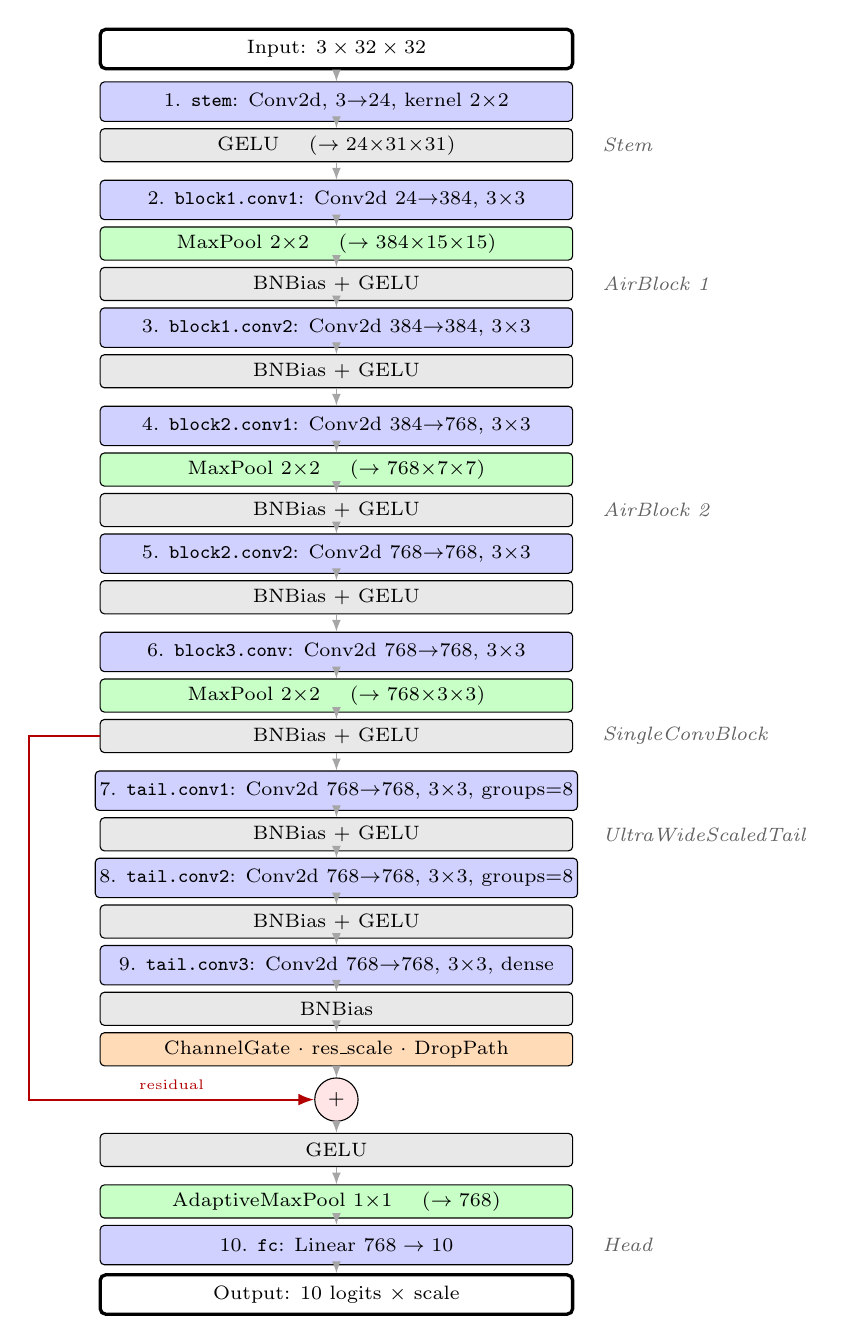
\begin{tikzpicture}[
    every node/.style={font=\scriptsize, align=center},
    conv/.style={draw, rectangle, rounded corners=1.5pt, fill=blue!18,
                 minimum width=6.0cm, minimum height=0.50cm, inner sep=1.5pt},
    bnact/.style={draw, rectangle, rounded corners=1.5pt, fill=gray!18,
                  minimum width=6.0cm, minimum height=0.42cm, inner sep=1.5pt},
    poolb/.style={draw, rectangle, rounded corners=1.5pt, fill=green!22,
                  minimum width=6.0cm, minimum height=0.42cm, inner sep=1.5pt},
    spec/.style={draw, rectangle, rounded corners=1.5pt, fill=orange!28,
                 minimum width=6.0cm, minimum height=0.42cm, inner sep=1.5pt},
    iobox/.style={draw, rectangle, rounded corners=2pt, fill=white,
                  minimum width=6.0cm, minimum height=0.50cm, inner sep=2pt, very thick},
    summer/.style={draw, circle, inner sep=1pt, fill=red!10, minimum size=0.55cm},
    grouplabel/.style={font=\scriptsize\itshape, color=gray!75!black},
    arrow/.style={-{Latex[length=1.5mm]}, thin, gray!70},
    resarrow/.style={-{Latex[length=2mm]}, thick, red!70!black}
]
\node[iobox] (input) {Input: $3 \times 32 \times 32$};
\node[conv, below=0.14cm of input] (stem) {1. \texttt{stem}: Conv2d, 3$\to$24, kernel 2$\times$2};
\node[bnact, below=0.08cm of stem] (sa) {GELU \quad ($\to 24{\times}31{\times}31$)};

\node[conv, below=0.22cm of sa] (b1c1) {2. \texttt{block1.conv1}: Conv2d 24$\to$384, 3$\times$3};
\node[poolb, below=0.08cm of b1c1] (b1p) {MaxPool 2$\times$2 \quad ($\to 384{\times}15{\times}15$)};
\node[bnact, below=0.08cm of b1p] (b1ba1) {BNBias + GELU};
\node[conv, below=0.08cm of b1ba1] (b1c2) {3. \texttt{block1.conv2}: Conv2d 384$\to$384, 3$\times$3};
\node[bnact, below=0.08cm of b1c2] (b1ba2) {BNBias + GELU};

\node[conv, below=0.22cm of b1ba2] (b2c1) {4. \texttt{block2.conv1}: Conv2d 384$\to$768, 3$\times$3};
\node[poolb, below=0.08cm of b2c1] (b2p) {MaxPool 2$\times$2 \quad ($\to 768{\times}7{\times}7$)};
\node[bnact, below=0.08cm of b2p] (b2ba1) {BNBias + GELU};
\node[conv, below=0.08cm of b2ba1] (b2c2) {5. \texttt{block2.conv2}: Conv2d 768$\to$768, 3$\times$3};
\node[bnact, below=0.08cm of b2c2] (b2ba2) {BNBias + GELU};

\node[conv, below=0.22cm of b2ba2] (b3c) {6. \texttt{block3.conv}: Conv2d 768$\to$768, 3$\times$3};
\node[poolb, below=0.08cm of b3c] (b3p) {MaxPool 2$\times$2 \quad ($\to 768{\times}3{\times}3$)};
\node[bnact, below=0.08cm of b3p] (b3ba) {BNBias + GELU};

\node[conv, below=0.22cm of b3ba] (tc1) {7. \texttt{tail.conv1}: Conv2d 768$\to$768, 3$\times$3, groups=8};
\node[bnact, below=0.08cm of tc1] (tba1) {BNBias + GELU};
\node[conv, below=0.08cm of tba1] (tc2) {8. \texttt{tail.conv2}: Conv2d 768$\to$768, 3$\times$3, groups=8};
\node[bnact, below=0.08cm of tc2] (tba2) {BNBias + GELU};
\node[conv, below=0.08cm of tba2] (tc3) {9. \texttt{tail.conv3}: Conv2d 768$\to$768, 3$\times$3, dense};
\node[bnact, below=0.08cm of tc3] (tn3) {BNBias};
\node[spec, below=0.08cm of tn3] (tg) {ChannelGate $\cdot$ res\_scale $\cdot$ DropPath};
\node[summer, below=0.14cm of tg] (sum) {$+$};
\node[bnact, below=0.14cm of sum] (ta3) {GELU};

\node[poolb, below=0.22cm of ta3] (gpool) {AdaptiveMaxPool $1{\times}1$ \quad ($\to 768$)};
\node[conv, below=0.08cm of gpool] (fc) {10. \texttt{fc}: Linear $768 \to 10$};
\node[iobox, below=0.10cm of fc] (out) {Output: 10 logits $\times$ scale};

\node[grouplabel, right=0.25cm of sa.east] {Stem};
\node[grouplabel, right=0.25cm of b1ba1.east] {AirBlock 1};
\node[grouplabel, right=0.25cm of b2ba1.east] {AirBlock 2};
\node[grouplabel, right=0.25cm of b3ba.east] {SingleConvBlock};
\node[grouplabel, right=0.25cm of tba1.east] {UltraWideScaledTail};
\node[grouplabel, right=0.25cm of fc.east] {Head};

\foreach \a/\b in {
    input/stem, stem/sa, sa/b1c1, b1c1/b1p, b1p/b1ba1, b1ba1/b1c2, b1c2/b1ba2,
    b1ba2/b2c1, b2c1/b2p, b2p/b2ba1, b2ba1/b2c2, b2c2/b2ba2,
    b2ba2/b3c, b3c/b3p, b3p/b3ba,
    b3ba/tc1, tc1/tba1, tba1/tc2, tc2/tba2, tba2/tc3, tc3/tn3, tn3/tg, tg/sum, sum/ta3,
    ta3/gpool, gpool/fc, fc/out}
    \draw[arrow] (\a) -- (\b);

\draw[resarrow] (b3ba.west) -- ++(-0.9,0) coordinate (rtop)
    -- (rtop |- sum.west) -- (sum.west)
    node[midway, above, sloped, font=\tiny, color=red!70!black] {residual};
\end{tikzpicture}
\label{fig:arch}
\end{figure}

\subsection{Reproducibility run instructions}

The final reproducibility script is configured from constants at the top of
\reprofile. On an 8-GPU RunPod A40 machine, the
current default runs 8 seeds in parallel, one seed per GPU:

\begin{verbatim}
python -u train_ultrawidescaledtail10_repro.py 2>&1 | tee full_8seed_run.log
\end{verbatim}

The default final configuration is:

\begin{center}
\begin{tabular}{ll}
\toprule
\textbf{Setting} & \textbf{Value} \\
\midrule
Seeds & 42 through 49 \\
Epochs per seed & 750 \\
Batch size & 128 \\
Seed workers & \texttt{auto}, resolving to 8 on an 8-GPU pod \\
DataLoader workers & 32 total, approximately 4 per seed process \\
Device layout & One independent training process per GPU \\
Output directory & \texttt{repro\_runs\_ultrawidescaledtail10\_8seed} \\
\bottomrule
\end{tabular}
\end{center}

The script first ensures that CIFAR-10 is available, then launches one process per GPU.
Each seed writes a checkpoint and JSON log. At the end, the script writes
\texttt{summary.csv} and \texttt{summary.json}.

\paragraph{Running on a single-GPU machine.}
The \texttt{"auto"} setting also handles single-GPU hardware: with one visible GPU,
the script runs the 8 seeds sequentially on that GPU, with no code change required.
However, each seed took about 93 minutes on an A40, so reproducing all 8 seeds
sequentially would take roughly 12 hours. To verify the pipeline in a much shorter
time, edit the constants at the top of
\reprofile to use a single seed:

\begin{verbatim}
RUN_SEEDS = (42,)
\end{verbatim}

This reduces the run to about 90 minutes on an A40-class GPU while still producing a
complete checkpoint, JSON log, and \texttt{summary.csv} entry for that seed. The same run
command is used in all cases:

\begin{verbatim}
python -u train_ultrawidescaledtail10_repro.py 2>&1 | tee full_8seed_run.log
\end{verbatim}

\subsection{Prior selection evidence}

Before the final 750-epoch run, I selected the model using prior 500-epoch
multi-seed evidence. Among the three strongest depth-limited single-model candidates,
\texttt{UltraWideScaledTail10} had the highest mean out-of-sample validation accuracy.
Ensemble artifacts in the parent experiment folder did score higher, but they combine
multiple checkpoints, so I left them out of the single-model result.

\begin{center}
\begin{tabular}{lrrrr}
\toprule
\textbf{Model} & \textbf{Seeds} & \textbf{Mean OOS Val.} & \textbf{Std.} & \textbf{Layers} \\
\midrule
\texttt{UltraWideScaledTail10} & 3 & 96.97 & 0.08 & 10 \\
\texttt{WideScaledPlus10} & 3 & 96.70 & 0.14 & 10 \\
\texttt{DeepScaled10} & 3 & 96.37 & 0.14 & 10 \\
\bottomrule
\end{tabular}
\end{center}

My retained seed-level evidence for the selected model was:

\begin{center}
\begin{tabular}{rrrrr}
\toprule
\textbf{Seed} & \textbf{Selected OOS Val.} & \textbf{Best Raw} & \textbf{Best EMA} & \textbf{Selected Epoch} \\
\midrule
42 & 96.94 & 96.88 & 96.94 & 459 \\
43 & 97.06 & 97.06 & 97.02 & 481 \\
44 & 96.90 & 96.90 & 96.90 & 486 \\
\bottomrule
\end{tabular}
\end{center}

The selected checkpoints occurred late in training, around epochs 459--486. This supports
the final decision to increase the reproducibility schedule to 750 epochs.

\subsection{Final 8-seed results}

The completed 8-seed RunPod sweep is summarized below from
\texttt{summary.csv}. The log file \texttt{full\_8seed\_run.log} confirms that all eight
seed jobs finished and wrote the sweep summary. The \texttt{test\_acc} column in the CSV
is blank because this run used validation selection only
(\texttt{RUN\_EVAL\_TEST\_AT\_END = False}).

\begin{center}
\begin{tabular}{rlrrrrr}
\toprule
\textbf{Seed} & \textbf{Ckpt.} & \textbf{Selected Val.} & \textbf{Epoch} &
\textbf{Best Raw} & \textbf{Best EMA} & \textbf{Wall Min.} \\
\midrule
42 & raw & 96.90 & 734 & 96.90@734 & 96.88@747 & 93.7 \\
43 & ema & 96.72 & 744 & 96.70@731 & 96.72@744 & 93.1 \\
44 & raw & 96.74 & 715 & 96.74@715 & 96.70@734 & 93.5 \\
45 & raw & 96.92 & 742 & 96.92@742 & 96.92@742 & 92.2 \\
46 & raw & 96.74 & 686 & 96.74@686 & 96.68@736 & 92.0 \\
47 & ema & 96.88 & 750 & 96.82@735 & 96.88@750 & 92.9 \\
48 & ema & 96.84 & 745 & 96.78@725 & 96.84@745 & 91.3 \\
49 & raw & 96.98 & 716 & 96.98@716 & 96.90@740 & 93.8 \\
\bottomrule
\end{tabular}
\end{center}

Across the eight seeds, the mean selected validation accuracy was 96.84\% with sample
standard deviation 0.10. The minimum selected validation accuracy was 96.72\%, the
maximum was 96.98\%, and the average per-seed wall time was 92.8 minutes. Broken out
by checkpoint type at each seed's best epoch, the average best-raw accuracy across the
eight seeds was 96.82\% and the average best-EMA accuracy across the eight seeds was
also 96.82\%. The per-seed mix, taking whichever of raw or EMA was higher for each
seed, averages to 96.84\%, matching the selected-validation mean.

\clearpage
\section{How and Why the Model Was Improved}

\Needspace{40\baselineskip}
I organized this section around the actual custom blocks in the final model. Each
block is shown in abbreviated code form, followed by the design reason and the alternative
that was rejected.

\subsection{Full architecture: wide trunk plus late residual tail}

\begin{lstlisting}[language=Python,caption={Submitted model skeleton}]
class UltraWideScaledTail10(nn.Module):
    def __init__(self, num_classes: int = 10, scale: float = 1 / 9):
        super().__init__()
        self.stem = nn.Conv2d(3, 24, kernel_size=2, padding=0, bias=True)
        self.stem_act = nn.GELU()
        self.block1 = AirBlock(24, 384, extra=False, pool=True)
        self.block2 = AirBlock(384, 768, extra=False, pool=True)
        self.block3 = SingleConvBlock(768, 768, pool=True)
        self.tail = UltraWideScaledTail(768)
        self.pool = nn.AdaptiveMaxPool2d(1)
        self.fc = nn.Linear(768, num_classes, bias=False)
        self.scale = scale

    def forward(self, x):
        x = self.stem_act(self.stem(x))
        x = self.block1(x)
        x = self.block2(x)
        x = self.block3(x)
        x = self.tail(x)
        x = self.pool(x).flatten(1)
        return self.fc(x) * self.scale
\end{lstlisting}

I made the model wider instead of deeper because the project has a strict
10-weighted-layer budget. Wide Residual Networks showed that increasing width can be a
better use of capacity than simply adding more depth on CIFAR-style tasks
\cite{zagoruyko2016wide}. The competing \texttt{DeepScaled10} model had fewer parameters
and more depth-like structure, but its 3-seed mean validation accuracy was lower
(96.37 versus 96.97). The selected architecture therefore spends the limited layer budget
on a high-capacity trunk and only adds extra refinement after the image has been reduced
to a small spatial map.

\Needspace{34\baselineskip}
\subsection{AirBlock and SingleConvBlock: simple convolutional trunk}

\begin{lstlisting}[language=Python,caption={Main trunk blocks}]
class AirBlock(nn.Module):
    def __init__(self, cin, cout, pool=True):
        super().__init__()
        self.conv1 = nn.Conv2d(cin, cout, 3, padding=1, bias=False)
        self.pool = nn.MaxPool2d(2) if pool else nn.Identity()
        self.bn1 = BNBias(cout)
        self.conv2 = nn.Conv2d(cout, cout, 3, padding=1, bias=False)
        self.bn2 = BNBias(cout)
        self.act = nn.GELU()

    def forward(self, x):
        x = self.act(self.bn1(self.pool(self.conv1(x))))
        return self.act(self.bn2(self.conv2(x)))

class SingleConvBlock(nn.Module):
    def __init__(self, cin, cout, pool=True):
        super().__init__()
        self.conv = nn.Conv2d(cin, cout, 3, padding=1, bias=False)
        self.pool = nn.MaxPool2d(2) if pool else nn.Identity()
        self.bn = BNBias(cout)
        self.act = nn.GELU()

    def forward(self, x):
        return self.act(self.bn(self.pool(self.conv(x))))
\end{lstlisting}

I used these blocks over transformer-style or MLP-style blocks because CIFAR-10 images
are small and local convolutional features are strong early in training. Pooling is
separate and parameter-free, so downsampling does not consume another weighted layer.
The activation is GELU rather than ReLU: ReLU is cheaper, but GELU gives a smooth
nonlinearity without adding parameters or counted layers \cite{hendrycks2016gelu}. This
was useful because the model has very few nonlinear stages under the layer limit.

\Needspace{14\baselineskip}
\subsection{BNBias: normalization without extra trainable scale}

\begin{lstlisting}[language=Python,caption={Frozen-scale batch normalization}]
class BNBias(nn.BatchNorm2d):
    def __init__(self, c: int, momentum: float = 0.4):
        super().__init__(c, momentum=momentum, affine=True)
        nn.init.ones_(self.weight)
        self.weight.requires_grad = False
\end{lstlisting}

\texttt{BNBias} keeps the stabilizing effect of batch normalization while freezing the
multiplicative scale parameter. Batch normalization is used because it improves
optimization by normalizing intermediate feature distributions \cite{ioffe2015batchnorm}.
I chose this over no normalization because the very wide layers were harder to train
stably without normalization. I also chose it over adding heavier normalization or
attention layers because the main capacity should stay in the counted convolutions.

\Needspace{18\baselineskip}
\subsection{ChannelGate: lightweight channel attention}

\begin{lstlisting}[language=Python,caption={ChannelGate}]
class ChannelGate(nn.Module):
    def __init__(self, channels: int, init_scale: float = 0.0):
        super().__init__()
        self.weight = nn.Parameter(torch.full((1, channels, 1, 1), init_scale))
        self.bias = nn.Parameter(torch.zeros(1, channels, 1, 1))

    def forward(self, x):
        avg = x.mean(dim=(2, 3), keepdim=True)
        scale = torch.sigmoid(avg * self.weight + self.bias)
        return x * (1.0 + scale)
\end{lstlisting}

I used this block instead of a full Squeeze-and-Excitation MLP. SE networks showed that
channel-wise recalibration can improve convolutional features \cite{hu2018senet}, but a
standard SE block would add extra \texttt{Linear} or \texttt{Conv2d} layers. Under my
layer-count rule, those layers would count against the model budget. \texttt{ChannelGate} keeps the useful idea,
global channel statistics controlling channel strength, while avoiding additional counted
weighted layers.

\Needspace{20\baselineskip}
\subsection{DropPath: residual-path regularization}

\begin{lstlisting}[language=Python,caption={DropPath}]
class DropPath(nn.Module):
    def __init__(self, drop_prob: float = 0.0):
        super().__init__()
        self.drop_prob = float(drop_prob)

    def forward(self, x):
        if self.drop_prob == 0.0 or not self.training:
            return x
        keep_prob = 1.0 - self.drop_prob
        shape = (x.shape[0],) + (1,) * (x.ndim - 1)
        mask = x.new_empty(shape).bernoulli_(keep_prob)
        return x * mask.div(keep_prob)
\end{lstlisting}

\texttt{DropPath} was my choice over ordinary dropout because the main overfitting risk is the
large residual tail, not a dense classifier head. Dropout reduces co-adaptation
\cite{hinton2012dropout,srivastava2014dropout}; stochastic depth applies the same idea
to residual branches \cite{huang2016stochasticdepth}. In this model, the residual tail is
randomly weakened during training while the full path is used at inference.

\Needspace{34\baselineskip}
\subsection{UltraWideScaledTail: grouped residual refinement}

\begin{lstlisting}[language=Python,caption={Low-resolution residual tail}]
class UltraWideScaledTail(nn.Module):
    def __init__(self, channels: int, groups: int = 8):
        super().__init__()
        self.conv1 = nn.Conv2d(channels, channels, 3, padding=1,
                               groups=groups, bias=False)
        self.bn1 = BNBias(channels)
        self.conv2 = nn.Conv2d(channels, channels, 3, padding=1,
                               groups=groups, bias=False)
        self.bn2 = BNBias(channels)
        self.conv3 = nn.Conv2d(channels, channels, 3, padding=1, bias=False)
        self.bn3 = BNBias(channels)
        self.res_scale = nn.Parameter(torch.zeros(1, channels, 1, 1))
        self.channel_gate = ChannelGate(channels)
        self.drop_path = DropPath(0.03)
        self.act = nn.GELU()

    def forward(self, x):
        residual = x
        x = self.act(self.bn1(self.conv1(x)))
        x = self.act(self.bn2(self.conv2(x)))
        x = self.bn3(self.conv3(x))
        x = self.channel_gate(x)
        return self.act(residual + self.drop_path(self.res_scale * x))
\end{lstlisting}

I placed the tail after the resolution has fallen to $768 \times 3 \times 3$. I chose
this over adding early high-resolution convolutions because late convolutions are much
cheaper in activation memory. The residual addition follows the ResNet idea of learning a
correction to an existing representation \cite{he2016resnet}. The first two tail
convolutions are grouped to reduce parameter and compute cost while retaining multiple
parallel transformations, following the ResNeXt cardinality idea \cite{xie2017resnext}.
The final dense convolution mixes information across all channels. The residual scale is
initialized at zero so the tail starts as a conservative correction instead of disrupting
the trunk at the start of training.

\Needspace{20\baselineskip}
\subsection{Initialization}

\begin{lstlisting}[language=Python,caption={Initialization pattern}]
def init_dirac_(conv: nn.Conv2d) -> None:
    nn.init.dirac_(conv.weight.data, groups=conv.groups)

def _apply_init(self) -> None:
    for block in (self.block1, self.block2):
        init_dirac_(block.conv1)
        init_dirac_(block.conv2)
    init_dirac_(self.block3.conv)
    init_dirac_(self.tail.conv1)
    init_dirac_(self.tail.conv2)
    init_dirac_(self.tail.conv3)
    nn.init.kaiming_normal_(self.fc.weight, nonlinearity="linear")
\end{lstlisting}

I used Dirac initialization for convolutional layers because it starts compatible
layers close to an identity-like mapping. This matches the residual design: begin from a
stable path and learn useful deviations. The classifier uses Kaiming initialization,
which was designed for deep rectifier networks and remains a standard initialization
choice for convolutional classifiers \cite{he2015rectifiers}.

\subsection{Training recipe choices}

\begin{center}
\begin{tabular}{p{0.25\linewidth}p{0.30\linewidth}p{0.35\linewidth}}
\toprule
\textbf{Technique} & \textbf{Used in script} & \textbf{Reason} \\
\midrule
RandAugment and random erasing & \texttt{RandAugment(2,14)} plus
\texttt{RandomErasing(p=0.25)} & Stronger image variation without a separate policy
search; random erasing forces less reliance on one local cue
\cite{cubuk2020randaugment,zhong2020randomerasing}. \\
Mixup & \texttt{RUN\_MIXUP = 0.2} & Smooths labels between examples and reduces
overconfident memorization \cite{zhang2018mixup}. \\
Label smoothing & \texttt{RUN\_LABEL\_SMOOTHING = 0.1} & Prevents the classifier from
training against fully hard one-hot targets \cite{szegedy2016inception}. \\
SGD with warmup and cosine decay & \texttt{SGD(..., nesterov=True)} with warmup cosine
schedule & Warmup avoids unstable early updates; cosine decay gives smaller late
updates for convergence \cite{goyal2017largebatch,loshchilov2017sgdr}. \\
EMA checkpointing & \texttt{AveragedModel(..., ema\_decay=0.999)} & Weight averaging
often improves validation stability and can select a flatter solution
\cite{izmailov2018swa,tarvainen2017meanteacher}. \\
Mixed precision and channels-last & CUDA bfloat16 autocast and channels-last tensors &
Improves GPU throughput and memory behavior without changing the architecture
\cite{micikevicius2018mixed,pytorchchannelslast}. \\
\bottomrule
\end{tabular}
\end{center}

\clearpage
\section{Attempts I Did Not Keep}

I tried or considered the following ideas during model development but did not
keep them in my final single-model submission. I included more than ten because they show the
iteration path, not just the final result. I treated these attempts as ablations: each
one tested whether a different way of spending the 10-layer budget would give a better
accuracy, simplicity, or reproducibility tradeoff.

\begingroup
\small
\renewcommand{\arraystretch}{1.15}
\begin{longtable}{r p{0.20\linewidth} p{0.32\linewidth} p{0.35\linewidth}}
\toprule
\textbf{\#} & \textbf{Attempt} & \textbf{What I was testing} &
\textbf{Why I did not keep it} \\
\midrule
\endhead
1 & \texttt{DeepScaled10} &
A more depth-oriented 10-layer candidate with fewer parameters than the final model. &
Its prior 3-seed mean validation accuracy was 96.37, below 96.97 for
\texttt{UltraWideScaledTail10}. This told me that extra depth-like structure was not as
valuable as width under the same layer limit. \\
2 & \texttt{WideScaledPlus10} &
A close 10-layer width-based alternative with a different scaling and tail balance. &
It was competitive, but its prior 3-seed mean was 96.70 with higher spread than the
selected model. I kept the stronger and more consistent \texttt{UltraWideScaledTail10}
result. \\
3 & Plain deeper scaling &
Using the limited layer budget to add more sequential transformations instead of
increasing channel capacity. &
The tests did not beat the width-first direction. With only 10 counted layers, every
extra convolution reduced the budget available for wide feature maps. \\
4 & Smaller parameter model preference &
Choosing the smaller model simply because it was lighter and easier to run. &
\texttt{DeepScaled10} was much smaller, but it gave lower validation accuracy. I decided
that parameter count alone was not the right objective as long as the final model still
fit the hardware and layer constraint. \\
5 & Historical \texttt{UltraWide7} &
An earlier 7-layer wide model that tested whether fewer counted layers could still get
close to the final accuracy. &
It reached 95.14 official test accuracy, which was useful progress but clearly below the
later 10-layer evidence. I used it as motivation to keep the wide trunk but spend the
remaining layers more carefully. \\
6 & Historical \texttt{WideScaled10} &
An earlier width-plus-tail 10-layer direction. &
It reached 94.83 official test accuracy, below later variants. The result suggested that
the general idea was promising, but the exact scaling and late tail needed improvement. \\
7 & \texttt{GhostScaled10} &
A compact ghost-style module intended to get cheaper feature expansion. &
It reached 94.52 official test accuracy and did not justify replacing the direct wide
convolutions. The cheaper module saved capacity, but the wide trunk learned stronger
CIFAR-10 features. \\
8 & \texttt{CoordAtt10} &
A coordinate-attention style model that tested whether explicit spatial/channel
attention would help enough to replace width. &
It also reached 94.52 official test accuracy. I did not keep it because the added
attention idea did not outperform the simpler wide convolutional trunk. \\
9 & Learned feature-concatenation ensemble &
Combining features from several trained models before classification. &
Did not respond to training as I hoped, I realized an ensamble of seperately trained
model would be better, but that would entail adding an 11th ensamble layer to the
ensamble of 10-Layer models. \\
10 & Weighted logit ensemble &
A simpler ensemble that combined model predictions rather than internal features. &
It improved complementarity, but it did not fit my single-model goal and exceeded the
strict total-layer interpretation. I kept the insight that the models made different
errors, but not the ensemble itself. \\
11 & Keeping all top-three models in the notebook &
Leaving \texttt{UltraWideScaledTail10}, \texttt{WideScaledPlus10}, and
\texttt{DeepScaled10} all in the final notebook. &
This slowed iteration and made the final comparison less focused. I streamlined the
notebook around the one model I actually selected, while reporting the others as
selection evidence. \\
12 & Short training as final evidence &
Using short runs to choose the final model and avoid long GPU sweeps. &
Short runs were useful smoke tests, but the selected checkpoints appeared around epochs
459--486 in prior evidence and around epochs 686--750 in the final 8-seed sweep. I
therefore used long training for the result I report. \\
\bottomrule
\end{longtable}
\endgroup

These attempts were useful because they narrowed the final design principle: within a
strict 10-layer budget, the best single model was not the deepest or smallest model, but
the model that combined a wide feature trunk with a low-resolution residual tail.

\section{Conclusion}

\texttt{UltraWideScaledTail10} is my final selected single model. It satisfies the
10-weighted-layer budget, has 21,337,656 parameters, and I selected it because it had the
best prior multi-seed out-of-sample validation performance among the tested single-model
candidates. I ran the final RunPod configuration for 8 seeds and 750 epochs on 8 A40 GPUs,
with one independent seed process per GPU.

\clearpage
\begin{thebibliography}{99}

\bibitem{he2016resnet}
K. He, X. Zhang, S. Ren, and J. Sun.
\newblock Deep Residual Learning for Image Recognition.
\newblock \emph{CVPR}, 2016.
\newblock \url{https://arxiv.org/abs/1512.03385}.

\bibitem{zagoruyko2016wide}
S. Zagoruyko and N. Komodakis.
\newblock Wide Residual Networks.
\newblock \emph{BMVC}, 2016.
\newblock \url{https://arxiv.org/abs/1605.07146}.

\bibitem{xie2017resnext}
S. Xie, R. Girshick, P. Dollar, Z. Tu, and K. He.
\newblock Aggregated Residual Transformations for Deep Neural Networks.
\newblock \emph{CVPR}, 2017.
\newblock \url{https://arxiv.org/abs/1611.05431}.

\bibitem{hu2018senet}
J. Hu, L. Shen, S. Albanie, G. Sun, and E. Wu.
\newblock Squeeze-and-Excitation Networks.
\newblock \emph{CVPR}, 2018.
\newblock \url{https://arxiv.org/abs/1709.01507}.

\bibitem{ioffe2015batchnorm}
S. Ioffe and C. Szegedy.
\newblock Batch Normalization: Accelerating Deep Network Training by Reducing
Internal Covariate Shift.
\newblock \emph{ICML}, 2015.
\newblock \url{https://arxiv.org/abs/1502.03167}.

\bibitem{hendrycks2016gelu}
D. Hendrycks and K. Gimpel.
\newblock Gaussian Error Linear Units (GELUs).
\newblock arXiv preprint, 2016.
\newblock \url{https://arxiv.org/abs/1606.08415}.

\bibitem{he2015rectifiers}
K. He, X. Zhang, S. Ren, and J. Sun.
\newblock Delving Deep into Rectifiers: Surpassing Human-Level Performance on
ImageNet Classification.
\newblock \emph{ICCV}, 2015.
\newblock \url{https://arxiv.org/abs/1502.01852}.

\bibitem{hinton2012dropout}
G. E. Hinton, N. Srivastava, A. Krizhevsky, I. Sutskever, and R. R. Salakhutdinov.
\newblock Improving Neural Networks by Preventing Co-adaptation of Feature
Detectors.
\newblock arXiv preprint, 2012.
\newblock \url{https://arxiv.org/abs/1207.0580}.

\bibitem{srivastava2014dropout}
N. Srivastava, G. Hinton, A. Krizhevsky, I. Sutskever, and R. Salakhutdinov.
\newblock Dropout: A Simple Way to Prevent Neural Networks from Overfitting.
\newblock \emph{Journal of Machine Learning Research}, 15:1929--1958, 2014.
\newblock \url{https://www.jmlr.org/papers/v15/srivastava14a.html}.

\bibitem{huang2016stochasticdepth}
G. Huang, Y. Sun, Z. Liu, D. Sedra, and K. Q. Weinberger.
\newblock Deep Networks with Stochastic Depth.
\newblock \emph{ECCV}, 2016.
\newblock \url{https://arxiv.org/abs/1603.09382}.

\bibitem{cubuk2020randaugment}
E. D. Cubuk, B. Zoph, J. Shlens, and Q. V. Le.
\newblock RandAugment: Practical Automated Data Augmentation with a Reduced
Search Space.
\newblock \emph{CVPR Workshops}, 2020.
\newblock \url{https://arxiv.org/abs/1909.13719}.

\bibitem{zhong2020randomerasing}
Z. Zhong, L. Zheng, G. Kang, S. Li, and Y. Yang.
\newblock Random Erasing Data Augmentation.
\newblock \emph{AAAI}, 2020.
\newblock \url{https://arxiv.org/abs/1708.04896}.

\bibitem{zhang2018mixup}
H. Zhang, M. Cisse, Y. N. Dauphin, and D. Lopez-Paz.
\newblock mixup: Beyond Empirical Risk Minimization.
\newblock \emph{ICLR}, 2018.
\newblock \url{https://arxiv.org/abs/1710.09412}.

\bibitem{szegedy2016inception}
C. Szegedy, V. Vanhoucke, S. Ioffe, J. Shlens, and Z. Wojna.
\newblock Rethinking the Inception Architecture for Computer Vision.
\newblock \emph{CVPR}, 2016.
\newblock \url{https://arxiv.org/abs/1512.00567}.

\bibitem{goyal2017largebatch}
P. Goyal, P. Dollar, R. Girshick, P. Noordhuis, L. Wesolowski, A. Kyrola,
A. Tulloch, Y. Jia, and K. He.
\newblock Accurate, Large Minibatch SGD: Training ImageNet in 1 Hour.
\newblock arXiv preprint, 2017.
\newblock \url{https://arxiv.org/abs/1706.02677}.

\bibitem{loshchilov2017sgdr}
I. Loshchilov and F. Hutter.
\newblock SGDR: Stochastic Gradient Descent with Warm Restarts.
\newblock \emph{ICLR}, 2017.
\newblock \url{https://arxiv.org/abs/1608.03983}.

\bibitem{izmailov2018swa}
P. Izmailov, D. Podoprikhin, T. Garipov, D. Vetrov, and A. G. Wilson.
\newblock Averaging Weights Leads to Wider Optima and Better Generalization.
\newblock \emph{UAI}, 2018.
\newblock \url{https://arxiv.org/abs/1803.05407}.

\bibitem{tarvainen2017meanteacher}
A. Tarvainen and H. Valpola.
\newblock Mean Teachers are Better Role Models: Weight-Averaged Consistency
Targets Improve Semi-Supervised Deep Learning Results.
\newblock \emph{NeurIPS}, 2017.
\newblock \url{https://arxiv.org/abs/1703.01780}.

\bibitem{micikevicius2018mixed}
P. Micikevicius, S. Narang, J. Alben, G. Diamos, E. Elsen, D. Garcia,
B. Ginsburg, M. Houston, O. Kuchaiev, G. Venkatesh, and H. Wu.
\newblock Mixed Precision Training.
\newblock \emph{ICLR}, 2018.
\newblock \url{https://openreview.net/pdf?id=r1gs9JgRZ}.

\bibitem{pytorchchannelslast}
PyTorch Contributors.
\newblock Channels Last Memory Format in PyTorch.
\newblock PyTorch documentation.
\newblock \url{https://docs.pytorch.org/tutorials/intermediate/memory_format_tutorial.html}.

\end{thebibliography}

\end{document}
